\section{\texttt{Experiments}}
\begin{frame}{\textbf{Experimental Setup}}
\begin{columns}
	\begin{column}{0.9\textwidth}
		\begin{varblock}[\textwidth]{UCF 50 Dataset}
			\begin{itemize}
				\item It has 50 classes with $\approx 5$ hours of training data.
				\item Contains video with diverse object appearance, object scale, viewpoint, cluttered background, illumination conditions, etc.
				\item Video classes are further grouped into body-motion (BM), human-object interaction (HOI), playing musical instruments (PI), indoor sports (IS) and outdoor sports.
			\end{itemize}
		\end{varblock}
	\end{column}	
\end{columns}
\end{frame}
\begin{frame}{\textbf{Approach I}}
\begin{columns}
	\begin{column}{0.6\textwidth}
	\begin{figure}
		\centering
		\fbox{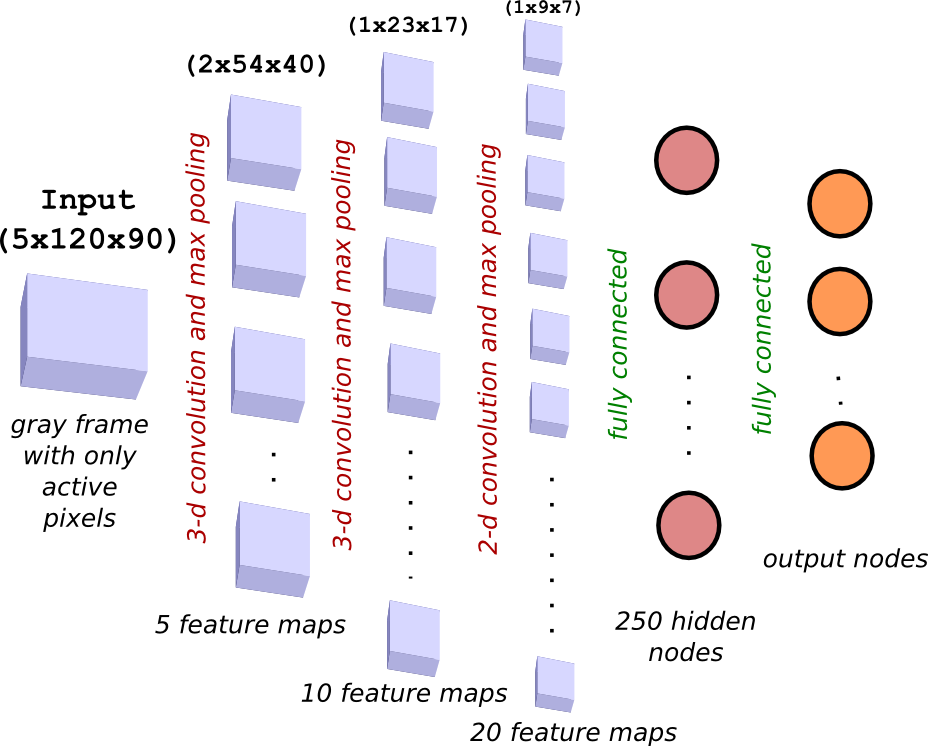
\includegraphics[height=0.7\textheight]{./img/cnn_config1.png}}
		\caption{CNN Architecture for Approach I}
	\end{figure}
	\end{column}
	\begin{column}{0.4\textwidth}
		\begin{itemize}
			\item Complete frame resized to $120 \times 90$ with inactive pixels masked.
			\item Only Gray channel.
		\end{itemize}
	\end{column}
\end{columns}
\end{frame}

\begin{frame}{\textbf{Approach II}}
\begin{columns}
	\begin{column}{0.6\textwidth}
	\begin{figure}
		\centering
		\fbox{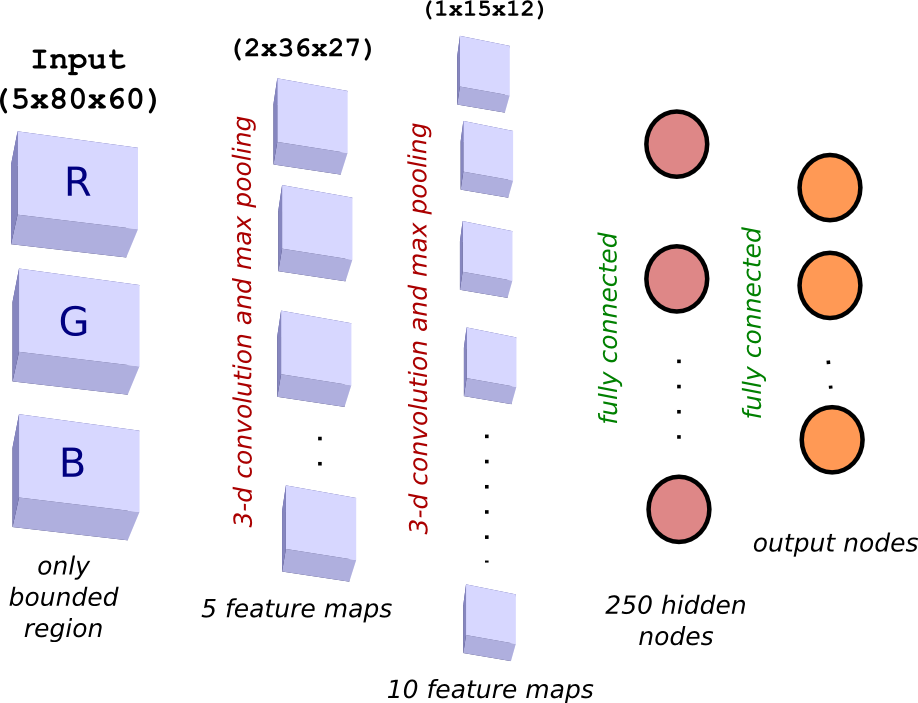
\includegraphics[height=0.7\textheight]{./img/cnn_config2.png}}
		\caption{CNN Architecture for Approach II}
	\end{figure}
	\end{column}
	\begin{column}{0.4\textwidth}
		\begin{itemize}
			\item Bounded regions are smartly resized to $80 \times 60$.
			\item All 3 Color channels.
		\end{itemize}
	\end{column}
\end{columns}
\end{frame}

\begin{frame}{\textbf{Approach III}}
\begin{columns}
	\begin{column}{0.6\textwidth}
	\begin{figure}
		\centering
		\fbox{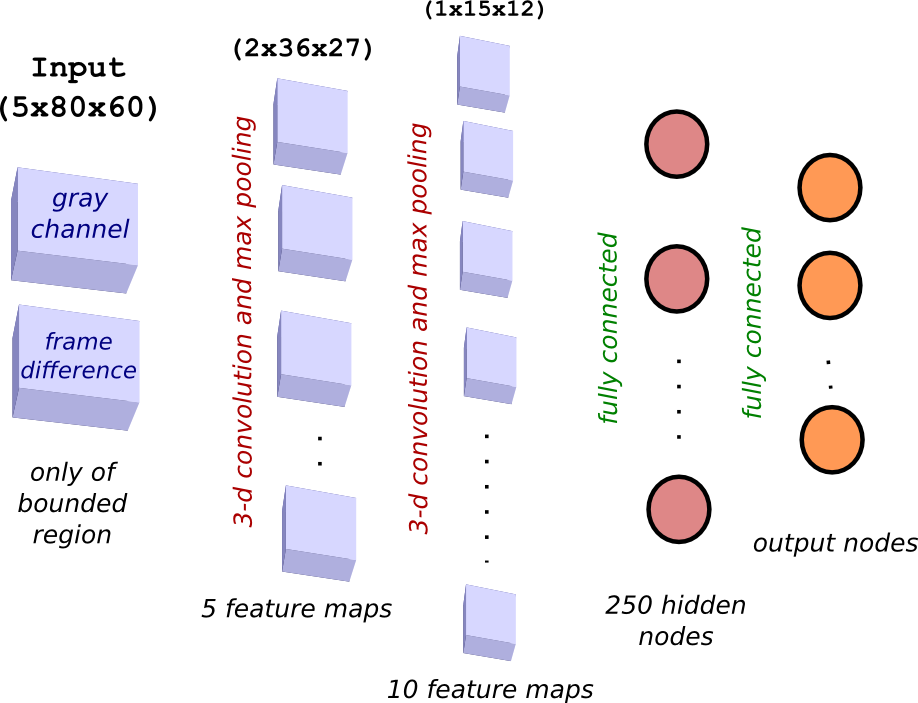
\includegraphics[height=0.7\textheight]{./img/cnn_config3.png}}
		\caption{CNN Architecture for Approach III}
	\end{figure}
	\end{column}
	\begin{column}{0.4\textwidth}
		\begin{itemize}
			\item Bounded regions are smartly resized to $80 \times 60$.
			\item Gray channel and Frame differencing.
		\end{itemize}
	\end{column}
\end{columns}
\end{frame}

\begin{frame}{\textbf{Results and Demo}}
	  \begin{scriptsize}
		\begin{table}[htbp]
		\caption{Test error (in $ \% $) on UCF 50 dataset}
			\begin{subtable}[Combined]{0.3\textwidth}
			\centering
			\caption{Combined}
			\begin{tabular}{|l|c|} \hline
				\textbf{Approach}&  \textbf{Combined} \\ \hline
        			I & 40.14\\ \hline
				II (with norm) &  {\color{yellow}\textbf{17.07}} \\ \hline		 
				III (with norm) &  25.23 \\ \hline
				\cite{recognizing50} &  33.26 \\ \hline
   			\end{tabular}
  	 	\end{subtable}
		\begin{subtable}[Individual groups]{0.6\textwidth}
			\centering
			\caption{Individual groups}			
			\begin{tabular}{|l|c|c|c|c|c|} \hline
        			\textbf{Approach} & \textbf{BM} & \textbf{HOI} & \textbf{PI} & \textbf{IS} & \textbf{OS} \\ \hline
				II & 8.63 & 3.85 & 1.36 & 2.21 & 9.21 \\ \hline
				II (with norm) & {\color{yellow}\textbf{8.51}} & {\color{yellow}\textbf{3.69}} & {\color{yellow}\textbf{1.33}} & {\color{yellow}\textbf{2.19}} & {\color{yellow}\textbf{9.08}} \\ \hline		 
				III (with norm) & 27.45 & 14.39 & 5.48 & 6.27 & 33.24 \\ \hline
  			 \end{tabular}
	   	\end{subtable}
 		\end{table} 
	\end{scriptsize}
	\begin{center}
		\fbox{\textbf{\color{black}Demo}}
		\begin{small}
		\begin{multicols}{3}
		\begin{itemize}
			\item BM~~{\color{red}[video]}
			\item HOI~~{\color{red}[video]}
			\item PI~~{\color{red}[video]}
			\item IS~~{\color{red}[video]}
			\item OS~~{\color{red}[video]}
			\item Combined~{\color{red}[video]}
		\end{itemize}
		\end{multicols}
		\end{small}
	\end{center}
\end{frame}

\section{\texttt{Conclusion}}
\begin{frame}{\textbf{Conclusion and Future Work}}
\begin{columns}
	\begin{column}{0.48\textwidth}
		\begin{varblock}[\textwidth]{Conclusion}
		\begin{itemize}
			\item Built deep neural network toolkit providing an ease to configure for different neural network models.
			\item Proposed a novel approach for video event localization by fusing the background subtraction and saliency measure to obtain better event classifier.
			\item Suggested appraoch for temporal smoothening is robust to sudden variations.
		\end{itemize}
		\end{varblock}
	\end{column}	
	\begin{column}{0.48\textwidth}
		\begin{varblock}[\textwidth]{Future Work}
		\begin{itemize}
			\item To revisit the indigenous convolutional neural network (CNN), to incorporate hierarchical learning. Layers will be trained in a way to discriminate the classes that were considered similar in the previous layer.
			\item Explore ways for associating the objects and events that are present
in the given video segment giving automated video annotation.
		\end{itemize}
		\end{varblock}
	\end{column}
\end{columns}
\end{frame}
\begin{frame}[plain]
	\begin{center}
	\begin{Huge}
		{\color{green}\texttt{THANKS}}
	\end{Huge}
	\end{center}
\end{frame}